\documentclass[12pt,titlepage]{article}
\usepackage{graphicx}
%\usepackage{graphics}
\usepackage{epsfig}
\usepackage{amsmath}
\usepackage{amssymb}
\usepackage{amsthm}
\usepackage{booktabs}
\usepackage{stmaryrd}
\usepackage{url}
%\usepackage{longtable}
\usepackage[figuresright]{rotating}
\usepackage{bigfoot}
\usepackage[titletoc,page]{appendix}
\usepackage{polski}
\usepackage[utf8]{inputenc}
\usepackage[T1]{fontenc}

\usepackage{geometry}
\usepackage{pslatex}
%\usepackage{ulem}

\usepackage{listings}
\usepackage{url}
%\usepackage{Here}
\usepackage{hyperref}
\hypersetup{
    colorlinks,
    citecolor=black,
    filecolor=black,
    linkcolor=black,
    urlcolor=black
}
\usepackage{color}
\usepackage{tcolorbox}
\tcbuselibrary{skins}
\renewcommand\appendixname{Dodatek}
\renewcommand\appendixpagename{Dodatki}
\colorlet{xlightblue}{blue!5}

\newtcolorbox{beamerlikethm}[1]{
  title=#1,
  beamer,
  colback=xlightblue,
  colframe=blue!30,
  fonttitle=\bfseries,
  left=1mm,
  right=1mm,
  top=1mm,
  bottom=1mm,
  middle=1mm
}

\definecolor{szary}{gray}{0.75}% jasnoszary

%\setlength{\textwidth}{400pt}

\lstset{numbers=left,
			numberstyle=\tiny, 
			basicstyle=\scriptsize\ttfamily, 
			breaklines=true, 
			captionpos=b, 
			tabsize=2}

\usepackage[ruled,vlined,linesnumbered]{algorithm2e}

\renewcommand*{\listalgorithmcfname}{Lista algorytmów}
\renewcommand*{\algorithmcfname}{Algorytm}
\renewcommand*{\algorithmautorefname}{Algorytm}

\vfuzz2pt % Don't report over-full v-boxes if over-edge is small
\hfuzz2pt % Don't report over-full h-boxes if over-edge is small


\newcommand{\RR}{\mathbb{R}}
\newcommand{\NN}{\mathbb{N}}
\newcommand{\QQ}{\mathbb{Q}}
\newcommand{\ZZ}{\mathbb{Z}}
\newcommand{\TAB}{\hspace{0.50cm}}
\newcommand{\IFF}{\leftrightarrow}
\newcommand{\IMP}{\rightarrow}

\newcommand{\PRZYKLAD}[1]{\par \noindent{\color{blue}PRZYKŁAD:}\\ {\color{szary}#1}\par}

\newtheorem{theorem}{Twierdzenie}[section]
\newtheorem{lemma}{Lemat}[section]
\newtheorem{example}{Przykład}[section]
\newtheorem{corollary}{Wniosek}[section]
\newtheorem{definition}{Definicja}[section]

\hyphenation{wszy-stkich ko-lu-mnę każ-da od-leg-łość
   dzie-dzi-ny dzie-dzi-na rów-nych rów-ny
   pole-ga zmie-nna pa-ra-met-rów wzo-rem po-cho-dzi
   o-trzy-ma wte-dy wa-run-ko-wych lo-gicz-nie
   skreś-la-na skreś-la-ną cał-ko-wi-tych wzo-rów po-rzą-dek po-rząd-kiem
   przy-kład pod-zbio-rów po-mię-dzy re-pre-zen-to-wa-ne
   rów-no-waż-ne bi-blio-te-kach wy-pro-wa-dza ma-te-ria-łów
   prze-ka-za-nym skoń-czo-nym mo-żesz na-tu-ral-na cią-gu tab-li-cy
   prze-ka-za-nej}


\begin{document}

\pagestyle{empty} %To jest strona tytułowa, bez numeracji

\begin{titlepage}
\vspace*{\fill}
\begin{center}
\begin{picture}(300,510)
  \put( 10,520){\makebox(0,0)[l]{\large \bf \textsc{Wydział Podstawowych Problemów Techniki}}}
  \put( 10,500){\makebox(0,0)[l]{\large \bf \textsc{Politechniki Wrocławskiej}}}
  \put( 10,315){\makebox(0,0)[l]{\Huge  \bf \textsc{Aplikacja do organizacji}}}
  \put( 10,290){\makebox(0,0)[l]{\Huge  \bf \textsc{imprez okolicznościowych}}}
  \put(100,240){\makebox(0,0)[l]{\large     \textsc{Jarosław Mirek}}}

  \put(170, 80){\makebox(0,0)[l]{\large  {Praca inżynierska napisana}}}
  \put(170, 60){\makebox(0,0)[l]{\large  {pod kierunkiem}}}
  \put(170, 40){\makebox(0,0)[l]{\large  {dr. inż. Marcina Zawady}}}

  \put(100,-80){\makebox(0,0)[bl]{\large \bf \textsc{Wrocław 2014}}}
\end{picture}
\end{center}
\vspace*{\fill}
\end{titlepage}

\tableofcontents

\newpage

\pagestyle{headings}  %Zaczynamy właściwą część dokumentu

\section*{Wstęp}      %* oznacza, że ta sekcja nie będzie numerowana   

Analizując kwestię planowania działań jednostki można dojść do wniosku, że społeczeństwo bardzo sprawnie radzi sobie z planowaniem krótko- oraz długoterminowym.
Nie jest dla nas problemem, aby określić co będziemy robić w nadchodzącym tygodniu lub, że w przeciągu pięciu lat skończymy studia i rozpoczniemy pierwszą pracę.
Kłopoty pojawiają się jednak podczas planowania w średnim terminie, czyli np. miesiąc, rok.

Okazuje się zatem, że w obliczu konieczności organizacji imprezy okolicznościowej (szczególnie formalnej) należy zadbać o wiele szczegółów, które razem mogą stanowić
nie lada wyzwanie planistyczne. Dodatkowo dosyć często jest to wyzwanie, przed którym stajemy właśnie w średnim terminie. Stąd potrzebne jest staranne rozplanowanie 
składowych wydarzenia, aby skutecznie je zorganizować w tym ograniczonym czasie.

Wraz z duchem czasu kartka i długopis odchodzą do lamusa, a my chcemy mieć stały dostęp do ``organizera'' naszego wydarzenia. Dlatego też idealnym rozwiązaniem
wydaje się być przeniesienie standardowego notesu do smartfona, w taki sposób, aby maksymalnie ułatwić kontrolę nad organizowanym wydarzeniem oraz usprawnić jego planowanie.
Przegląd rynku aplikacji smartfonowych pokazuje, że systemy służące organizacji wydarzeń są nastawione na konkretny typ okoliczności np. wesele lub nieformalną imprezę.
Istnieje jednak luka dla aplikacji, która:

\begin{itemize}
 \item posłuży do organizacji różnego typu wydarzeń,
 \item pozwoli organizować zarówno wydarzenia o charakterze bardzo uroczystym, jak i te nieformalne,
 \item zintegruje wszystkich uczestników wydarzenia,
 \item wyręczy organizatora w części obowiązków.
\end{itemize}


W związku z powyższym, celem zrealizowanej pracy dyplomowej było zaprojektowanie oraz implementacja systemu w modelu klient-serwer dedykowanemu systemowi operacyjnemu Android.
System jest w stanie wspomóc organizację imprezy okolicznościowej na kilku płaszczyznach, a wymagania funkcjonalne były następujące:

\begin{itemize}
 \item wspieranie organizacji bardzo uroczystych wydarzeń, jak i tych nieformalnych,
 \item skupienie wokół wydarzenia wszystkich jego uczestników,
 \item możliwość deklaracji uczestników na prezenty lub rzeczy,
 \item skoncentrowanie ważnych elementów imprezy (kontakty, notatki, listy rzeczy do zrobienia) w aplikacji.
\end{itemize}

Jako system o zbliżonej funkcjonalności można przytoczyć serwis Facebook, wraz z oferowaną przezeń funkcjonalnością wydarzeń.
Facebook'owe wydarzenia mają jednak przede wszystkim funkcjonalność informacyjną oraz służą za miejsce do wymiany myśli przez zaproszonych użytkowników.
Zrealizowany projekt rozszerza jednak znacznie ten pomysł, dodając możliwość jednoznacznej deklaracji uczestników, co do kwestii, którymi się zajmą.
Ponadto system oferuje funkcjonalności stricte planistyczne, dzięki którym organizator w formie ``kreatora'', zostanie poprowadzony przez proces pozwalający 
skutecznie zaplanować imprezę okolicznościową.

Niniejsza praca składa się z czterech rozdziałów. W pierwszym rozdziale omawiamy dokładniej problem, oraz sposób interakcji użytkowników ze sobą, a także
przypadki użycia aplikacji.

Rozdział drugi zawiera szczegółowy projekt systemu. Opiszemy w nim poszczególne komponenty składające się na całość zaimplementowanej aplikacji. Przeanalizujemy
aplikację kliencką, stronę serwera, a także bazę danych i komunikację pomiędzy tymi składowymi. Zawrzemy w nim również opis algorytmu generowania unikalnego i losowego
kodu, który jest kluczem dostępu gości do wydarzenia.

Rozdział trzeci uszczegółowi użyte technologie oraz pewne kwestie implementacyjne, którymi cechuje się napisany system.

Czwarty rozdział dotyczyć będzie tematu wdrożenia systemu, natomiast rozdział końcowy podsumuje otrzymane wyniki, związane z nimi możliwe kierunki rozwoju,
a także wypunktuje powodzenie implementacyjne systemu.

\newpage
\section{Analiza problemu}
W tym rozdziale zajmiemy się przede wszystkim tym, co charakteryzuje problem wykonania aplikacji mobilnej w modelu klient-serwer dla tematu naszej pracy. Zawrzemy w nim
ponadto sposób podziału ról pomiędzy użytkownikami oraz zmianą struktury aplikacji w zależności od typu organizowanego wydarzenia.

Dla ustalenia uwagi rozdział ten rozpoczniemy od zagadnienia, z którego wyrósł pomysł stworzenia opisywanego w pracy systemu:

\begin{beamerlikethm}{}
Zwyczajowo para, która planuje zawrzeć związek małżeński organizuje przyjęcie weselne. Jednym z nierozerwalnych elementów takiego wydarzenia są prezenty.
Niekiedy młoda para tworzy listę prezentów, które chciałaby otrzymać od gości, a listę taką najczęściej dzierży świadek i to on nadzoruje całe przedsięwzięcie
oraz deklaracje gości dotyczące kupna danego przedmiotu. Nie jest to jednak zbyt wygodna forma, ponieważ goście nie zawsze mają możliwość dokładnego przeanalizowania
listy, a nadzorca listy musi poświęcić swój czas dużej ilości gości. Ponadto mogą pojawić się niedogodności komunikacyjne, które zaowocują duplikatem prezentu. Wady można
jeszcze mnożyć. Dlaczego więc nie pomyśleć o liście prezentów w interaktywnej, cyfrowej formie? Wystarczy dodatkowa karteczka dołączona do zaproszenia, wraz z kodem
oraz instrukcją dotyczącą jego użycia.
\end{beamerlikethm}

Przyjęcie weselne to jednak nie tylko prezenty, ale także mnóstwo obowiązków organizacyjnych, setki telefonów i formalności. Jeśli jednak głębiej się zastanowimy
te same problemy dotyczą organizacji bankietu, urodzin czy nawet nieformalnej uroczystości, które jest współorganizowane przez wszystkich uczestników.

Stąd też jeśli nasza aplikacja ma tym problemom zaradzić, to musimy rozważyć kilka istotnych zagadnień:

\begin{enumerate}
 \item Użytkownicy i ich role:
 \\ Przede wszystkim musimy podzielić użytkowników na organizatorów i uczestników.
 Organizator to użytkownik, który decyduje czy wydarzenie ma charakter oficjalny, czy też nie, ustala listę gości, definiuje listę prezentów (lub, w przypadku
 nieformalnej, współorganizowanej imprezy, przedmioty/dania/napoje, które sa potrzebne), a także powinien móc zdefiniować listę spraw, które należy dopełnić czy też
 posiadać prosty skorowidz, umożliwiający kontakt z firmami zajmującymi się salą, cateringiem czy orkiestrą. Powinien on także posiadać funkcjonalności uczestnika.
 
 Uczestnik jest natomiast użytkownikiem, który może wskutek zalogowania kodem wydarzenia przejrzeć jego szczegóły, tj. gdzie i kiedy się odbędzie czy też listę gości.
 Dodatkowo uczestnik może w formie systemu komentarzy toczyć dyskusję dotyczącą wydarzenia, a także zadeklarować chęć zakupu prezentu z listy.
 
 \item Tajność wydarzenia
 \\ Wydarzenie powinno być przedmiotem zainteresowania uczestniczących w nim gości. Wszelkie szczegóły nie powinny być dostępne każdemu użytkownikowi aplikacji, a jedynie
 osobom, które organizator mianował uczestnikami. Rozwiązaniem, które zostało wymyślone na potrzeby aplikacji jest losowy, unikalny kod, który pozwoli zalogować się do
 wydarzenia. Organizator, tworząc uroczystość w systemie otrzyma stosowny ciąg alfanumeryczny, które może później przekazać zainteresowanym.
 
 
 \item Weryfikacja użytkowników
 \\ System kodu logującego tworzy możliwość, że użytkownik wpisując losowo ciąg cyfr i znaków alfabetu zaloguje się do jakiegoś wydarzenia, którego uczestnikiem być nie powinien.
 Stąd też należy zadbać o weryfikację użytkowników. Z pomocą przychodzi konto w portalu Facebook. W tej chwili bardzo dużo osób posiada takie konto, dzięki czemu można bardzo łatwo
 zweryfikować kim jest zalogowany w aplikacji użytkownik.
 Oprócz tego uniemożliwia to wtargnięcie w kompetencje organizatora.
 
 \item Stworzenie części serwerowej
 \\ System, który w założeniach ma integrować użytkowników o różnych rolach musi posiadać zdalny komponent, który będzie przechowywał wpisywane do systemu informacje
 oraz odpowiednio je propagował pomiędzy nimi. Serwer powinien zatem być zintegrowany z bazą danych oraz umożliwiać prostą komunikację ze smartfonem.
\end{enumerate}


Ważnym elementem systemu z podziałem ról jest również taki projekt aplikacji, który pozwoli na dynamiczną zmianę funkcjonalności w zależności od typu użytkownika. Uczestnik
nie powinien być w stanie dodawać prezentów do listy, a od organizatora nie oczekuje się możliwości deklaracji na prezent, który sam ma otrzymać. Stąd też w naszym systemie
należało stworzyć aplikację, która połączy widoki dla obu ról, oraz serwer, który odpowiednio roześle dane.

Przechodząc do analizy komunikacji pomiędzy aplikacją mobilną, a serwerem należało zastanowić się w jaki sposób przesyłać dane. Dodatkowo należało zaprojektować integrację
serwera z bazą danych tak, aby te trzy komponenty niezawodnie współpracowały, reagowały na nietypowe zdarzenia i były bezpieczne.

Ostatecznym elementem, który w decydujący sposób wpłynąłby na sukces komercyjny systemu jest interfejs użytkownika aplikacji klienckiej. Funkcjonalna aplikacja wymaga, aby
jego interfejs nie wymagał przedzierania się przez gąszcz ekranów, a jego składowe powinny mieć intuicyjny charakter, ew. wsparty elementem pomocy, jaką można uzyskać w odpowiednim
miejscu.

\newpage
\section{Projekt systemu}
W tej części pracy zajmiemy się szczegółowym opisem komponentów odpowiadających za całość systemu. Opiszemy w jaki sposób komponenty te współpracują ze sobą, a także 
poruszymy kwestie związane z komunikacją i algorytmami wymaganymi do sprawnego funkcjonowania systemu.

\subsection{Założenia}
W założeniach system składa się z czterech komponentów: strony internetowej, aplikacji mobilnej oraz serwera zintegrowanego z bazą danych.

\begin{itemize} % to trzeba bedzie przejrzec w zaleznosci od tego jak potoczy sie ze strona
 \item Strona internetowa powinna oferować możliwość integracji posiadanego przez użytkownika konta Facebook z aplikacją kliencką.
 Po zintegrowaniu konta można rozpocząć użytkowanie aplikacji mobilnej. Powinna także zawierać te same funkcjonalności co aplikacja mobilna.
 \item Aplikacja mobilna to element, który pozwoli na pobieranie i przesyłanie danych użytkowników do serwera. Pozwoli również edytować, przetwarzać i umieszczać
dane na ekranie urządzenia. 
 \item Serwer to serce aplikacji. Najważniejszy element systemu, który powinien identyfikować użytkowników, dbać o prawidłową propagację danych, jak również
 sprawnie współpracować ze zintegrowaną bazą danych.
 \item Baza danych, to komponent, w którym przechowywane są wszystkie informacje użytkowników. Ponadto zawiera ona informacje związane z systemem logowania użytkowników do systemu.
\end{itemize}

\subsection{Architektura systemu}
System jest oparty o tzw. model ``klient-serwer''. Oznacza to, że istnieje centralne miejsce w systemie (serwer), które operuje na wszystkich danych, przetwarza je, zapamiętuje, a także w odpowiednim
formacie rozsyła do klientów. W takim modelu element klienta służy przede wszystkim do komponowania zapytań do serwera i wyświetlania zwracanych danych.

W naszym projekcie za komponent kliencki rozumiemy aplikację mobilną oraz stronę internetową. Są to elementy o zbliżonej funkcjonalności. Serwer ma natomiast obsługiwać zapytania dla obu tych technologii.
Ponadto serwer ma działać zdalnie ze z góry określonymi funkcjonalnościami, jakie oferuje system.
Nasz projekt jest generalnie oparty o tworzenie wydarzeń, które skupiają konkretne grupy użytkowników. Wobec tego chcemy, aby serwer był wspólny dla różnych wydarzeń i aby jego utrzymanie i administracja
leżała w gestii usługodawcy systemu.
Jak już wspomnieliśmy wcześniej baza danych zawiera wszystkie informacje z systemu, toteż zakłada się, że będzie ona silnie zintegrowana z serwerem. Chcemy, aby użytkownik, który ma styczność
z aplikacją kliencką mógł jej skutecznie używać bez potrzeby znajomości architektury systemu, czy też sposobu komunikacji.

%napisze tu jeszcze o integracji z baza danych, oraz komunikacja, a takze ze serwer obsluguje i strone i androida. moze cos jeszcze

\subsection{Aplikacja mobilna}
W tej, jak i kilku kolejnych części dokumentu opiszemy to, jak na etapie projektu powinny wyglądać funkcjonalności poszczególnych elementów systemu. Rozpoczniemy od aplikacji mobilnej.

Jak już wspomnieliśmy wcześniej aplikacja mobilna dedykowana jest systemowi operacyjnemu Android. Stąd też kluczowym słowem będzie tzw. Aktywność (Activity). Szerzej o technicznych aspektach
systemu Android wspomnimy w rozdziale dedykowanym opisom technologii. Na tym etapie o Aktywności należy myśleć jako o pojedynczym widoku w aplikacji smartfonowej, który posiada pewne funkcjonalności
pozwalające użytkownikowi na interakcje z aplikacją.

Jednym z kluczowych celów opisywanego systemu było to, żeby aplikacja mobilna miała przyjazny interfejs użytkownika. Stąd też projektując system chcielibyśmy, aby miał on ``płytki'' charakter.
Mamy tu na myśli, że nie trzeba przejść wielu Aktywności, aby dojść do najbardziej zagnieżdżonej funkcjonalności aplikacji.

\begin{figure}
\begin{center}
 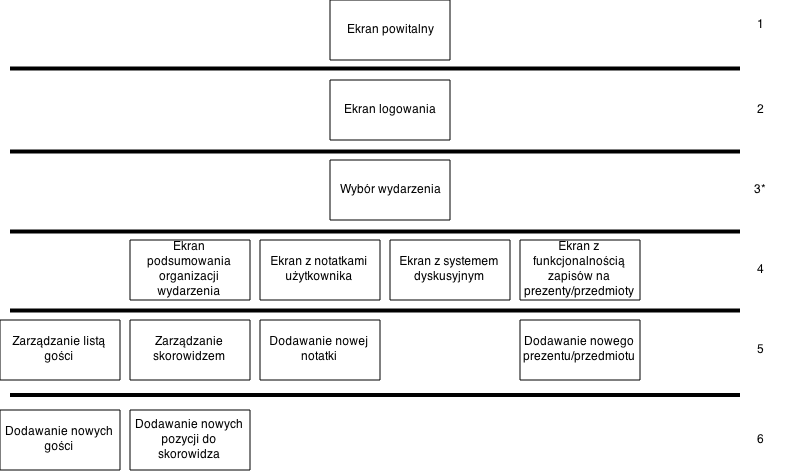
\includegraphics[scale=0.5]{/home/lagvna/Dokumenty/inz_gfx/funk.png}
 \caption{Diagram przedstawiający poziomy funkcjonalności w aplikacji mobilnej}
 \label{fig:funk}
\end{center}
\end{figure}

Można to przeanalizować bardziej szczegółowo, spoglądając na rysunek~\ref{fig:funk}. Aplikacja ma sześć poziomów zagnieżdżenia. Oznacza to, że należy dokonać co najwyżej 5 dotknięć ekranu 
(włącznie z uruchomieniem) i co najwyżej trzech przesunięć palcem po ekranie, aby dojść do dowolnej funkcjonalności. Poziom nr 3 oznaczyliśmy gwiazdką, ponieważ zależy ona od aktora.
W przypadku gdy użytkownik jest organizatorem, to być może organizuje kilka wydarzeń jednocześnie, stąd należało przewidzieć wybór, administracji którego chce się aktualnie podjąć.
Dla gościa poziom ten nie jest wymagany, ponieważ wydarzenia są jednoznacznie identyfikowane kodem dostępu. Wobec czego podając otrzymany od organizatora ciąg alfanumeryczny system
sam dołączy gościa do odpowiedniego wydarzenia.
Dodatkowo czynności, które polegają na dodawaniu informacji do systemu, nie będą udostępniane gościom. Jedynym wyjątkiem jest tutaj możliwość deklaracji zakupu prezentu lub przedmiotu
na nadchodzące wydarzenie. Względnie toczenie dyskusji na ekranie z systemem temu poświęconym.

Wszystko to czyni, że aplikacja ma prosty interfejs, który skupia się wokół poziomu nr 4. 
W tym miejscu mamy bowiem cztery najważniejsze funkcje w aplikacji, współistniejące obok siebie, dzięki możliwościom jakie niesie system Android. Oferuje on rozwiązanie w postaci
tzw. zakładek, czyli jednej aktywności, która łączy w sobie kilka widoków (tzw. fragmentów), przy czym nawigacja polega na przesuwaniu palcem po ekranie odpowiednio w lewą lub prawą stronę. 
To właśnie ten pomysł jest sednem w kwestii projektu ``płytkiej'' nawigacji po aplikacji.

Będąc przy Rysunku~\ref{fig:funk} możemy od razu przeanalizować aplikację pod kątem projektowanych funkcjonalności:

\begin{itemize}
 \item Poziom 1.
      \begin{itemize}
        \item Ekran powitalny.
        \\Jest to ekran, który widzimy tuż po uruchomieniu aplikacji. To widok, który przedstawia logo i nazwę aplikacji, pozostaje na ekranie przez kilka sekund, po czym samoczynnie
        znika na rzecz kolejnego poziomu w aplikacji.
       \end{itemize}
 \item Poziom 2.
       \begin{itemize}
        \item Ekran logowania.
        \\ W tym miejscu użytkownik ma szansę rozpocząć interakcję z oprogramowaniem. W tej aktywności użytkownik może zalogować się do aplikacji swoim kontem Facebook.
        Po uwierzytelnieniu odblokowane zostaną przyciski pozwalające na dokonanie wyboru czy użytkownik chce utworzyć swoje wydarzenie, czy też planuje zalogować się
        do już istniejącego, którego kod dostępu posiada.
       \end{itemize}
 \item Poziom 3*.
      \begin{itemize}
       \item Wybór wydarzenia.
       \\ Jak już opisaliśmy wcześniej jest to wyłącznie funkcjonalność organizatora, który może administrować więcej niż jedno wydarzenie jednocześnie. Z tego względu powinien móc
       zdecydować, którym zająć się w danym momencie. W przypadku, gdy organizator chce utworzyć nowe wydarzenie, ma szansę również zrobić to z tego poziomu aplikacji, podając kilka podstawowych
       informacji, takich jak: nazwa, miejsce, data czy krótki opis.
      \end{itemize}
 \item Poziom 4.
      \begin{itemize}
       \item Ekran podsumowania organizacji wydarzenia.
       \\Jest to element aplikacji, który zawiera podstawowe informacje o wydarzeniu: nazwa, data, miejsce, krótki opis. Dodatkowo pozwala przejść do niższych poziomów interfejsu,
       związanych z listą gości oraz skorowidzem organizatora.
       \item Ekran z notatkami użytkownika.
       \\Organizacja wydarzenia (szczególnie oficjalnej) wymaga zadbania o wiele szczegółów. Aplikacja zaoferuje więc funkcjonalność notatek, wraz z tzw. elementem
       zatwierdzania już wykonanych zadań. Ma to być swoisty notes, do którego dostęp ma jedynie organizator.
       \item Ekran z systemem dyskusyjnym.
       \\W tym miejscu mamy komponent pozwalający na wymianę myśli uczestników wydarzenia. W założeniach ma to być uproszczone forum, przypominające Facebook'owy system komentarzy.
       \item Ekran z funkcjonalnością zapisów na prezenty/przedmioty.
       \\W przypadku oficjalnych imprez takich jak wesele, organizator może życzyć sobie ustalenia listy prezentów, które chciałby otrzymać od uczestników. Wobec tego w tym miejscu
       może on obserwować jak przebiegają zapisy gości na zadeklarowane przez niego przedmioty.
       W ramach imprezy nieformalnej często jest ona współorganizowana przez gości. Wymaga to wielu przygotowań i obowiązków, które dobrze byłoby rozdzielić pomiędzy nich. 
       Dlatego też jest to idealne miejsce dla tego typu wymagań.
       Warto również podkreślić, że funkcjonalność dodawania pozycji dla powyższej funkcjonalności, leży w uprawnieniach organizatora i została przewidziana dla poziomu 5.
      \end{itemize}
 \item Poziom 5.
      \begin{itemize}
	\item Zarządzanie listą gości.
	\\W tym miejscu można przejrzeć listę gości, którą organizator przewidział w ramach wydarzenia. Funkcjonalność ta pozwoli w łatwy sposób skontaktować się z danym gościem (e-mail, numer telefonu).
	\item Zarządzanie skorowidzem.
	\\Przy organizacji wydarzenia często zaangażowane są w to zewnętrzne firmy, zajmujące się specjalistyczną branżą. Ta funkcjonalność pozwoli na szybki kontakt.
	\item Dodawanie nowej notatki.
	\\Notatki to funkcjonalność przewidziana wyłącznie dla organizatora. Powinien on móc dodawać nowe notatki, wraz z kolejnymi etapami organizacji. Aby ułatwić nieco wprowadzanie danych
	funkcjonalność ta znajduje się w kolejnym poziomie i posiadać będzie swoją aktywność.
	\item Dodawanie nowego prezentu/przedmiotu.
	\\Prezenty wymagają podania szczegółów dotyczących zakupu - link do sklepu internetowego, nazwa, opis, zakres cenowy. Stąd dodawanie nowego przedmiotu zostało zniesione do niższego poziomu,
	aby poprawić ergonomię funkcjonalności.
      \end{itemize}
 \item Poziom 6.
      \begin{itemize}
       \item Dodawanie nowych gości.
       \\Jest to funkcjonalność pozwalająca na dodanie gościa do listy wraz ze szczegółami kontaktowymi, tj. adresem e-mail oraz numerem telefonu (opcjonalnie).
       \item Dodawanie nowych pozycji do skorowidza.
       \\Podobnie jak w przypadku gości, skorowidz powinien oferować szczegóły kontaktowe, które należy wprowadzić w oddzielnym ekranie aplikacji.
      \end{itemize}
      
\end{itemize}

\subsection{Aplikacja internetowa}
W tym podrozdziale przejdziemy do kolejnego komponentu systemu, jakim jest serwis internetowy.
W założeniach aplikacja internetowa powinna posiadać te same funkcjonalności, co aplikacja mobilna, stąd poświęcimy tu tylko niewielki fragment, w których ujmiemy główne wytyczne tego elementu. 

Smartfony są bardzo wygodnymi urządzeniami wyświetlającymi informacje. Niemniej jednak ich wprowadzanie za pomocą klawiatury systemu Android może już być dosyć kłopotliwe, 
nawet jeśli myślimy o urządzeniach posiadających dużą przekątną ekranu (np. tablet). Jest to szczególnie dotkliwym problemem, jeśli rozważymy konieczność dodania kilkudziesięciu 
osób do listy gości, wraz z numerami telefonów oraz adresami e-mail.
Dlatego też strona internetowa powinna być tym elementem systemu, który pozwoli ułatwić użytkownikowi wprowadzania danych do systemu z poziomu komputera osobistego, ale także wygodne
ich przeglądanie. W poprzednim podrozdziale bardzo szczegółowo potraktowaliśmy opis funkcjonalności aplikacji mobilnej. W przypadku aplikacji internetowej chcemy wykonać wierną kopię 
wraz z opisywanym założeniem ``płytkości'' nawigacji, w celu zapewnienia ergonomii systemu.

Należy również podkreślić, że w przypadku strony internetowej uwierzytelnianie będzie odbywać się także za pomocą konta Facebook, które użytkownik już musi posiadać, aby zacząć korzystać
z aplikacji.

Na koniec chcemy również przypomnieć, że aplikacja internetowa powinna być obsługiwana przez ten sam serwer, co aplikacja mobilna. Zapewni to synchronizację przepływu danych pomiędzy klientami,
korzystającymi z różnych platform, jak również oszczędności finansowe w chwili gdybyśmy rozpoczęli rozważania nad komercyjnym wdrożeniem systemu.

\subsection{Projekt serwera}
W tej części pracy omówimy to, w jaki sposób powinien działać projektowany w systemie serwer, jak będzie rozgraniczał komunikację pomiędzy aplikacją mobilną, a internetową, a także w jaki sposób
zostanie on zintegrowany z bazą danych.

Chociaż wspominaliśmy w podrozdziale dotyczącym założeń projektowanego systemu, że serwer to najważniejsza część aplikacji, to jest to wbrew pozorom dość prosty komponent.
Cykl działania serwera powinien wyglądać w następujący sposób:

\begin{enumerate}
 \item Serwer otrzymuje zapytanie od klienta,
 \item Serwer sprawdza, czy klient jest uwierzytelniony,
 \item Jeśli nie, to odsyła informację o niepowodzeniu i koniec,
 \item Jeśli tak, to:
 \subitem [W przypadku zapytania o informacje z bazy danych] serwer wykonuje zapytanie do bazy danych pod kątem informacji, o które pyta klient,
 \subitem [W przypadku wprowadzania nowych informacji do bazy danych] serwer parsuje dane od klienta i dodaje odpowiednią krotkę do bazy danych,
 \item Serwer przetwarza dane, aby opakować je w ustalony dla komunikacji sposób (w naszym przypadku będzie to format JSON, o czym mowa w odpowiednim podrozdziale),
 \item Serwer odsyła dane klientowi i koniec.
\end{enumerate}

Jak widać chodzi nam przede wszystkim o to, aby serwer działał w prosty sposób. Ponadto mamy następujące wymagania odnośnie serwera:

\begin{itemize}
 \item bezpieczeństwo,
 \item niezawodność,
 \item możliwość współpracy z zewnętrznym kontem (u nas Facebook),
 \item szybkość działania,
 \item możliwość rozwijania systemu.
\end{itemize}

W związku z tym w projektowanym systemie zdecydowaliśmy się wykorzystać istniejące rozwiązanie jakim jest wysokopoziomowy framework przeznaczony do tworzenia aplikacji internetowych napisanym w Pythonie,
czyli Django\footnote{\verb|https://www.djangoproject.com/|}. Szerzej narzędzie to opiszemy w odpowiednim rozdziale. Niemniej na tym etapie należy wspomnieć, że Django opiera się na 
wzorcu projektowym Model-View-Template\footnote{\verb|https://docs.djangoproject.com/en/1.7/faq/general/|}, dzięki czemu charakteryzuje się bardzo modułowym sposobem tworzenia aplikacji.
W momencie kiedy mamy już model (czyli tak naprawdę tabelę bazy danych), wystarczy napisać odpowiedni widok, który jest pewnego rodzaju funkcją uruchamianą po nadejściu zapytania od klienta.
Funkcja ta wyciąga zadane informacje z bazy danych, następnie opakowuje do uzgodnionego formatu i odsyła klientowi. Dzięki temu chcąc nadać systemowi nową funkcjonalność nie ma konieczności
ingerowania w już istniejące. Poza tym Django, jako narzędzie cały czas rozwijane cechuje się wysoką wydajnością, bezpieczeństwem, a także wygodą użytkowania. Django generuje automatycznie panel
administratorski, wspiera różnego rodzaju wtyczki, dzięki czemu można do aplikacji logować się kontem społecznościowym, jak również oferuje serwer deweloperski do testowania aplikacji.

Nasz serwer działa w taki sposób, że każda funkcja (widok) jest niejako zduplikowana. Wynika to z konieczności obsłużenia dwóch rodzajów klientów: smartfona oraz przeglądarki internetowej.
W przypadku tego pierwszego chcemy móc wygodnie parsować dane, co wiąże się z koniecznością przesyłania ich w odpowiednim formacie. Zdecydowaliśmy się na JSON, z którym Android radzi sobie bardzo dobrze.
W kwestii przeglądarki internetowej dane chcemy od razu wyświetlać w docelowym otoczeniu czyli szablonie strony internetowej.

Ważna jest też integracja z bazą danych. Domyślnie Django (w zintegrowany sposób) wspiera system SQLite, który jest dużo wydajniejszy przy obsłudze jednego użytkownika od np. MySQL, czy PostreSQL.
Skrypty tworzące bazę danych leżą po stronie mechanizmów framework'u, oraz unikamy konieczności pisania zapytań do bazy danych, którymi ten również się zajmuje.

\subsection{Projekt bazy danych}

\begin{figure}[htb]
\begin{center}
 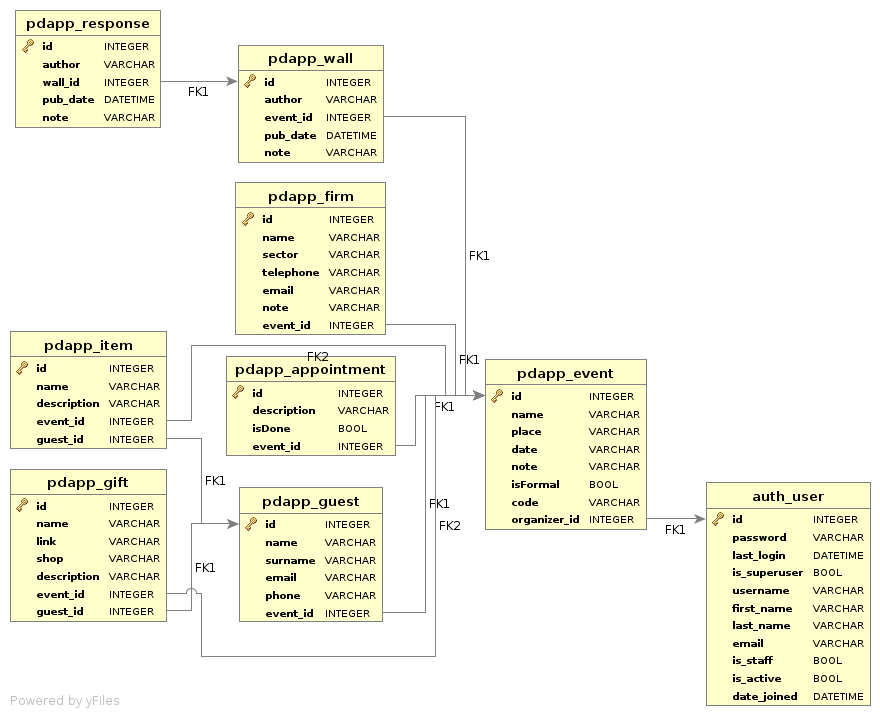
\includegraphics[scale=0.42]{/home/lagvna/Dokumenty/inz_gfx/dbpart.png}
 \caption{Diagram przedstawiający schemat bazy danych serwera}
 \label{fig:dbpart}
\end{center}
\end{figure}
\newpage
W tym podrozdziale zajmiemy się dokładniejszym omówieniem bazy danych, w ujęciu funkcjonalności systemu oraz potrzeby silnej jej integracji z serwerem, o czym wspominaliśmy w poprzednich częściach
pracy. Z tego też względu, dla ustalenia uwagi, rozpoczęliśmy od rysunku~\ref{fig:dbpart}, do którego będziemy się odwoływać.

Zaprojektowane przez nas w bazie danych tabele dotyczą:

\begin{enumerate}
 \item Wydarzenia (\textbf{pdapp\_event})
 \item Gości (\textbf{pdapp\_guest})
 \item Kontaktu ze skorowidza (\textbf{pdapp\_firm})
 \item Tablicy dyskusyjnej (\textbf{pdapp\_wall})
 \item Odpowiedzi w wątku tablicy dyskusyjnej (\textbf{pdapp\_response})
 \item Spraw do załatwienia (\textbf{pdapp\_appointment})
 \item Prezentu/Przedmiotu (\textbf{pdapp\_gift})
\end{enumerate}

Oprócz powyższych mamy jeszcze tabelę \textbf{auth\_user}. Jest to tabela generowana przez mechanizm uwierzytelniania użytkowników przez serwer. Jednak umieściliśmy ją na Rysunku~\ref{fig:dbpart}, 
dla pełniejszego zrozumienia kompozycji bazy danych.
Ponadto w Dodatku~\ref{sec:dball} zaprezentowano cały schemat bazy danych jakim posługuje się serwer. Tabele te są wynikiem wbudowanego w serwer Django mechanizmu uwierzytelniania i autoryzacji, a także
obsługi logowania za pomocą kont społecznościowych przez wtyczkę Allauth\footnote{\verb|http://www.intenct.nl/projects/django-allauth/|}.

Omówimy teraz pokrótce wypunktowane tabele:

\begin{itemize}
 \item[Ad 1.] Wydarzenia to centralna tabela bazy danych. Konkretna krotka należy do organizatora. Posiada pola opisujące nazwę, datę, miejsce, oraz krótki opis.
 \item[Ad 2.] Goście przynależą do danego wydarzenia. Jest to jednak lista kontaktowa organizatora, w której wyróżniamy między innymi numer telefonu oraz e-mail.
 \item[Ad 3.] Kontakty w założeniach mają opisywać dane firm obsługujących wydarzenie.
 \item[Ad 4.] Tablica dyskusyjna to tzw. wpisy główne. Przyrównując do forum, powiedzielibyśmy, że to wątki.
 \item[Ad 5.] Celem tej tabeli jest przypisanie odpowiedzi w dyskusji do wątków.
 \item[Ad 6.] Sprawy do załatwienia opisują wspomniane w podrozdziale o funkcjonalnościach aplikacji mobilnej notatki organizatora.
 \item[Ad 7.] Rekordy systemu zapisów na prezenty/przedmioty (odpowiednio: wydarzenie formalne/nieformalne).
\end{itemize}

Całość pozwala obsłużyć wszystkie zaprojektowane dla aplikacji klienckich funkcjonalności. Dodatkowo baza danych zachowuje przy takiej budowie prostotę oraz możliwość dalszej rozbudowy
w przypadku dodawania do systemu nowych funkcjonalności.

\subsection{Opis komunikacji} %moze tu jeszcze dorzucic diagram ten co z prezentacji u Klonowskiego?
Aby połączyć ze sobą wszystkie komponenty systemu należało zaprojektować ustalony sposób porozumiewania, aby dane mogły sprawnie przepływać. Dlatego też opiszemy w jaki sposób aplikacje
klienckie pytają serwer o dane, oraz jak ten odpowiada na żądania.

W przypadku aplikacji mobilnej komunikacja z serwerem odbywa się poprzez tekstowy format JSON. Wynika to z faktu, że jest to format, który zajmuje mało miejsca w porównaniu z innymi rozwiązaniami.
Jest to także proste i czytelne rozwiązanie, bowiem obiekt JSON to zbiór elementów typu klucz-wartość.
\begin{beamerlikethm}{Przykład obiektu typu JSON}
\{``name'': ``Jarek'', ``surname'': ``Mirek'', ``phone'': ``505404303''\}
\end{beamerlikethm}
Co istotne nasza aplikacja kliencka ma charakter online, wobec czego wszystkie informacje są na bieżąco pobierane przez sieć internetową, stąd chcieliśmy aby sumarycznie zminimalizować ich ilość.
W takiej sytuacji JSON był odpowiednim rozwiązaniem, szczególnie w konfrontacji np. z formatem XML.

Przejdźmy teraz do aplikacji internetowej, w której komunikacja jest kwestią bardzo przyjemną. Jak już wspominaliśmy Django używa wzorca projektowego Model-View-Template. 
Ten ostatni człon stanowi o miejscu wyświetlania danych serwera. Template to nic innego jak strona internetowa napisana w języku HTML, jednak Django oferuje nam wpisywanie 
w kodzie słów kluczowych (specjalnie dla niego przewidzianych), wyświetlających dane z bazy danych, które to później tłumaczy na standardowy język HTML. 
To kolejna zaleta stosowanego rozwiązania, ponieważ pozwala stworzyć dynamiczny serwis internetowy przy oszczędności nakładów pracy i dba za nas o komunikację, gdyż jest to część serwera.

\subsection{Opis algorytmu generowania losowego, unikalnego kodu}
Bardzo ważnym aspektem implementowanego systemu jest generowanie losowego, unikalnego ciągu alfanumerycznego. Jest to o tyle istotne, że projekt zakłada, iż każde wydarzenie jest jednoznacznie
skorelowane z takim kodem. Dzięki temu osoba, która otrzyma kod od organizatora loguje się za pomocą aplikacji klienckiej tylko i wyłącznie przy jego użyciu. Takie podejście jest wygodne,
ale i zarazem stanowi pewne wyzwanie projektowe.

Przeanalizujmy wobec tego możliwe podejścia:

\begin{itemize}
 \item Załóżmy, że chcemy wygenerować kod pięcioznakowy, który posiada dwie cyfry, oraz trzy litery. Jednym z podejść jest wylosowanie niezależnie cyfr i liter, a następnie ustalenie
 (również w drodze losowania), na której pozycji powinny znaleźć się poszczególne typy znaków. Następnym krokiem jest sprawdzenie czy w bazie danych istnieje już wylosowany kod. W przypadku
 duplikatu procedurę powtarzamy.
 
 \item Kolejny pomysł polega na koncepcji wygenerowania wszystkich możliwych kodów pięcioznakowych i trzymanie ich np. w jakimś pliku. Teraz wystarczyłoby już tylko w trybie krokowym
 uruchomić algorytm permutacji Fischer-Yate's:
 
 {\small
\begin{algorithm}[H]
%\SetAlTitleFnt{small}
\SetArgSty{normalfont}
\SetKwInOut{Input}{Wejście}
\SetKwInOut{Output}{Wyjście}
\Input{Tablica kodów K}
\For{$i \leftarrow |K|$ \KwTo $1$}{
$j \leftarrow $ losowa liczba naturalna taka, że $0 \leqslant j \leqslant i$; \

$ swap(K[i], K[j])$;}
\caption{Algorytm permutacji Fischer-Yate's}\label{alg:fyp}
\end{algorithm}
}

Oznacza to mniej więcej tyle, że w każdym kolejnym kroku pozycja, na którą aktualnie wskazuje zmienna iterująca jest już ustawiona i to ją możemy przypisać nowoutworzonemu wydarzeniu.

\item Ostatnim pomysłem jest użycie symetrycznego szyfru blokowego np. DES i, przy jednakowym kluczu, szyfrowanie kolejnych liczb naturalnych, rozpoczynając od danej wartości.

\end{itemize}

Ostatnie podejście wydaje się być dobrym, jeśli mamy dużą dziedzinę i potrzebujemy bardzo wielu kodów. Trzeba jednak wziąć pod uwagę, że rozwiązanie to mogłoby zacząć przynosić duplikaty
kodów, w momencie gdy przekroczymy pewien próg szyfrowanych wartości, przy założeniu o pięcioznakowości kodów.

Permutacja Fischer-Yate's jest bardzo dobrym rozwiązaniem w przypadku gdy żądamy wielkiej ilości kodów przy małej mocy zbioru argumentów. Kłopotliwym jednak wydaje się być konieczność posiadania
pewnej bazy kodów od samego początku.

Pierwsze podejście jest optymalne dla stosunkowo niewielkiej liczby kodów z dużej dziedziny. W naszym przypadku (2 cyfry, 3 litery i losowe ich ustawienie) zbiór argumentów liczy:
$ \binom{5}{2} \cdot 10 \cdot 10 \cdot 26 \cdot 26 \cdot 26 \approx 17,5$ mln elementów. Oznacza to, że prawdopodobieństwo powtórzenia jest małe, nawet jeśli wykorzystamy już setki tysięcy kodów. Niemniej jednak
w razie takiej sytuacji mamy zabezpieczenie w postaci powtórnego losowania. Ponadto mechanizm ten jest prosty w implementacji oraz nie ma potrzeby ustalania kluczy, generowania plików itp.
Biorąc pod uwagę wszystkie argumenty zdecydowaliśmy się wykorzystać w systemie właśnie takie podejście.

% moze tutaj jeszcze dodac listing jak to robie? jak bede mial :p
\newpage
\section{Implementacja sytemu} 
W tym rozdziale zaprezentujemy technologie, jakie zostały użyte w systemie. Omówimy czym się charakteryzują oraz w jaki sposób działają. Oprócz tego powiemy co sprawiło trudności 
w implementacji systemu, a jakie decyzje (podjęte jeszcze w fazie projektu) pozwoliły uzyskać zadowalający efekt prosto i szybko.
\subsection{Opis technologii}
\subsubsection{Aplikacja mobilna}
Jak już wspomnieliśmy wcześniej aplikacja mobilna dedykowana jest systemowi operacyjnemu Android. Platformą docelową są więc nowoczesne smartfony.
Oprogramowanie dla takich urządzeń pisze się w języku JAVA, jednak Android oferuje bardzo bogate biblioteki, które pozwalają na interakcje z urządzeniem docelowym.

Technologia ta cechuje się rozdzieleniem graficznego interfejsu użytkownika, zasobów oraz logiki aplikacji. Dwa pierwsze pisze się za pomocą struktury XML w odpowiednich plikach.
Następnie pliki te ``podpina'' się do części logicznej aplikacji (pisanej, jak już wspomnieliśmy, w języku JAVA) za pomocą odpowiednich identyfikatorów i adapterów, wbudowanych w biblioteki Androida.
Technologia ta jest bardzo wygodna w użyciu, gdyż praca nad aplikacją ma modułowy charakter. Każdy ekran aplikacji to osobna klasa dziedzicząca po tzw. Activity. W niej definiujemy akcje podejmowane
po naciśnięciu odpowiednich elementów interfejsu, lub po wprowadzeniu danych.

Warto jeszcze wspomnieć, że Android oferuje wtyczki do takich środowisk programistycznych jak Eclipse. Posiada także emulator, dzięki czemu nie jest konieczne posiadanie fizycznego urządzenia, aby
rozwijać oprogramowanie.
\subsubsection{Aplikacja internetowa}
Rozwijanie atrakcyjnych aplikacji internetowych wymaga wiedzy i doświadczenia, niemniej jednak kluczem do sukcesu jest talent i pewien zmysł estetyczny. Na szczęście istnieją bardzo wygodne narzędzia,
pozwalające w prosty sposób wykonać jak najatrakcyjniejszy produkt. W naszym projekcie skorzystaliśmy Bootsrap.

Jest to framework twórców Twittera, który w istocie tworzy zbiór gotowych rozwiązań HTML i CSS stanowiących elementy do budowy całości strony. Dzięki temu komponując poszczególne składowe ze sobą,
jesteśmy w stanie:

\begin{itemize}
 \item stworzyć responsywny serwis internetowy, czyli taki, który zapewni optymalny wygląd strony niezależnie od rozdzielczości i innych parametrów,
 \item skorzystać z wielu komponentów, dzięki czemu nie musimy samodzielnie pisać formularzy czy ramek,
 \item wykonać strony, które równie dobrze wyglądają w przeglądarce komputera osobistego, jak i na ekranie smartfona czy tabletu.
\end{itemize}

Myśląc o komercyjnym wykorzystaniu projektu skorzystanie z Bootstrap, oprócz oczywistego ułatwienia pracy nad projektem, pozwola na proste dokonywanie zmian, 
czy też zmianę szablonów stron.
\subsubsection{Serwer aplikacji}
W rozdziale dotyczącym projektu systemu wspominaliśmy już, że serwer aplikacji jest oparty o Django. W tym miejscu powiemy jednak nieco szerzej czym cechuje się
to narzędzie.

Przypomnijmy, że Django to framework służący do tworzenia aplikacji internetowych, który przy pomocy wzorca projektowego Model-View-Template pozwala tworzyć dynamiczne serwisy
internetowe w bardzo efektywny sposób. Model możemy identyfikować w Django z bazą danych. Niemniej cała obsługa tejże leży po stronie silnika Django, a my definiujemy jedynie
tabele, ich kolumny oraz wzajemne relacje pomiędzy nimi. 

Mając już model, Django oferuje mechanizm tzw. widoków (View). Widok to swojego rodzaju funkcja, która uruchamiana jest za pomocą
wejścia pod odpowiedni adres. W funkcji tej można przefiltrować dane z bazy, pod kątem interesujących nas informacji, a następnie wysłać do szablonu (Template). Używany do pisania wspomnianych widoków
język to Python. Warto jeszcze wspomnieć, że zarządzanie adresami podstron jest również w opisywanym framework'u bardzo ułatwione. Wystarczy w odpowiednim pliku zdefiniować nazwę odnośnika 
i zadeklarować jaki widok uruchamia.

Szablony w Django (Template) to tak naprawdę pliki HTML, które pozwalają na wstawianie specjalnego kodu źródłowego, dzięki czemu dane wyfiltrowane w widoku można umieścić w żądanym miejscu.
To pozwala na tworzenie dynamicznej zawartości, a przy tym nie wymaga od nas rozbudowywania serwisu o dziesiątki dodatkowych plików.

Przypomnijmy, że w naszym systemie komunikacja z aplikacją mobilną odbywa się przy pomocy obiektów typu JSON. W Django do tworzenia widoków używamy Python'a, wobec czego mamy dostęp do bibliotek
jakie język ten oferuje. Stąd bardzo łatwo jest użyć Django na różnych platformach, bo mamy dostęp do narzędzi, które tworzą i parsują JSON'y.
\subsection{Szczegóły implementacyjne}


W początkowej fazie problematycznym wyzwaniem była implementacja uwierzytelniania użytkowników za pomocą konta Facebook. Wprawdzie istnieje wiele wtyczek dla Django, które oferują taką funkcjonalność,
niemniej jednak wiele z nich żąda od użytkownika informacji prywatnych z Facebook'a. Z tego względu użytkownik z nieprawidłowymi względem wtyczki ustawieniami konta nie miałby możliwości autoryzacji.
Ostatecznie dobrym rozwiązaniem okazała się wtyczka Allauth, jednak dokumentacja tego narzędzia jest bardzo skromna i pojawiły się problemy z jego integracją z projektem serwera.
\begin{figure}[htb]
 \begin{center}
 
\includegraphics[scale=0.4]{/home/lagvna/Dokumenty/inz_gfx/logo.png}
 \caption{Logo stworzonego systemu}
 \label{fig:logo}
 \end{center}
\end{figure}

Pomijając jednak te początkowe trudności wybór Django jako serwera systemu okazał się świetnym rozwiązaniem, bowiem prostota jego użycia skróciła znacznie implementację. Dodatkowo wzorzec
projektowy jakim się posługuje pozwolił na wykonanie centralnego serwera, który obsługuje zarówno aplikację internetową, jak i tę mobilną. Ponadto w przypadku konieczności nadania nowych
funkcjonalności systemowi, to właśnie serwer będzie wymagał najmniej zmian.

Użycie Bootstrap'a okazało się również trafnym wyborem, ponieważ końcowy efekt cechuje się schludnym i funkcjonalnym szablonem, a wraz z użyciem Django okazał się nie wymagać wielkich nakładów
czasowych.

Najwięcej pracy wymagała implementacja aplikacji mobilnej. Należało ręcznie napisać wiele widoków oraz całą logikę programu. Ponadto aplikacja nieustannie komunikuje się z serwerem, 
więc należało zaimplementować porozumiewanie się modułów za pomocą zdarzeń asynchronicznych, których w kodzie źródłowym można znaleźć wiele. Stanowiło to trudność wymagającą dobrego zrozumienia
jak wygląda cykl komunikacyjny, oraz synchronizacji wątków pomiędzy sobą.

Konkludując należy jednak uznać, że wynikiem pracy jest sukces implementacyjny, a stworzone oprogramowanie działa bez zarzutów oraz spełnia wymagania funkcjonalne, oraz cele wyznaczone w fazie projektowej.
\newpage
\section{Instalacja systemu}
W rozdziale tym opiszemy wymagania co do środowiska oraz instrukcję jak uruchomić projekt załączony do ninejszej pracy na płycie, w celu testowania.
Warto odnieść się przy tej okazji do Dodatku~\ref{sec:cd}, który zawiera opis zawartości płyty.

Rozpoczniemy od wymagań dotyczących środowiska uruchomieniowego:

\begin{itemize}
 \item System operacyjny Linux,
 \item Środowisko Java SE Development Kit 8
 \item Zintegrowane środowisko programistyczne Eclipse, wydanie Luna,
 \item Wtyczka Android SDK Tools w wersji 23.0.5 dla Eclipse,
 \item Framework Bootstrap,
 \item Telefon z systemem Android w wersji $\geqslant$ 4.0 lub odpowiednia maszyna wirtualna Android,
 \item Aktywne konto na portalu społecznościowym Facebook.
\end{itemize}

Po spełnieniu powyższych wymagań możemy przejść do opisu sposobu uruchomienia poszczególnych komponentów:

\begin{enumerate}
 \item \textbf{Serwer dewelopersji Django, wraz ze stroną internetową:}
 \\Po rozpakowaniu pliku \verb|serwer.zip| w dogodnym miejscu na dysku komputera, należy uruchomić terminal i przejść do katalogu \verb|serwer/PerfectDay/|, w którym znajduje się projekt serwera.
 Teraz należy użyć komendy:
 \begin{center}
  \verb|$python manage.py runserver|
 \end{center}
Po tej operacji można już swobodnie rozpocząć korzystanie ze strony internetowej aplikacji.
W tym celu należy uruchomić przeglądarkę internetową i odwiedzić za jej pomocą adres: \verb|http://127.0.0.1:8000|.
\newpage
\item \textbf{Aplikacja mobilna:}
\begin{beamerlikethm}{Uwagi!}
W celu sprawnego testowania aplikacji mobilnej należy uruchomić serwer deweloperski Django (patrz krok 1.).
\\Przed przystąpieniem do konfiguracji należy poznać adres IP komputera, na którym uruchomiony jest serwer. Jeśli telefon działa w tej samej sieci, co serwer wystarczy wewnętrzny adres.
W przypadku różnych sieci, potrzebować będziemy zewnętrznego adresu IP.
\\Ponadto należy zadbać o odblokowanie portu 8000 (router, firewall itp.).
\end{beamerlikethm}

\begin{itemize}
 \item Po rozpakowaniu pliku \verb|klient.zip| w dogodnym miejscu na dysku komputera należy uruchomić środowisko Eclipse ze skonfigurowaną wtyczką Android SDK.
Następnie należy kliknąć \verb|File->Import...|, a następnie wybrać \verb|Existing Android Code Into Workspace|. Dalej wystarczy kliknąć \verb|Browse| w górnej części okienka i wskazać ścieżkę, 
w które znajduje się projekt tj. \verb|klient/PerfectDay|. Następnie musimy zatwierdzić wybór i kliknąć \verb|Finish| w dolnej części okna.
\item Po tej operacji należy w środowisku Eclipse i zaimportowanym projekcie odszukać plik \verb|LoginActivity.java|, w którym potrzeba zedytować linię metody \verb|OnCreate|
otoczoną czerwoną ramką na rysunku~\ref{fig:ip}
\begin{figure}[htb]
\begin{center}
 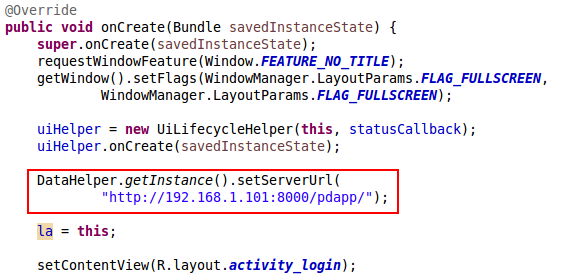
\includegraphics[scale=0.6]{/home/lagvna/Dokumenty/inz_gfx/ipconfig.png}
 \caption{Linia, w której edytujemy IP serwera, do którego łączy się aplikacja}
 \label{fig:ip}
 \end{center}
\end{figure}

Należy w tym miejscu podać adres IP serwera, pod którym działa serwer deweloperski Django.

\item Po pomyślnej edycji adresu IP należy zapisać plik i skompilować projekt, uruchamiając go na smartfonie lub w maszynie wirtualnej Androida.
\end{itemize}

\end{enumerate}


\newpage
\section*{Podsumowanie}
Chcąc podsumować ninejszą pracę, a także omawiany w niej system należy wyjść od faktu, że udało się spełnić zakładane w fazie projektowej funkcjonalności i cele.
To, co zasługuje na szczególną uwagę to:
\begin{itemize}
 \item serwer, który obsługuje aplikację mobilną i internetową jednocześnie,
 \item aplikacja kliencka, posiadająca ``płytki'' interfejs użytkownika (dostęp do każdej funkcjonalności aplikacji),
 \item utożsamienie wydarzenia z unikalnym, losowym kodem, dzięki czemu nie jest konieczne wpisywanie dużych ilości informacji, aby się zalogować,
 \item praktyczne wykorzystanie i integracja technologii i rozwiązań wysokiego poziomu (Android, Bootstrap, Django, Facebook).
\end{itemize}
To wszystko czyni, że system jest nie tylko ukończony, ale i przygotowany do uruchomienia w szerszej społeczności. Przy tej okazji warto podkreślić fakt, że oprogramowanie
wymaga pewnego rodzaju pielęgnacji. Mowa tu o usuwaniu starych wydarzeń, co pozwoli na rzadsze pojawianie się duplikatów podczas generowania kodu wydarzenia.
Alternatywnie można z góry ustalić, jakie wydarzenia kwalifikujemy jako stare i rozwinąć serwer o mechanizm, który będzie to robić automatycznie.

Mimo, że opisywany w pracy system jest kompletnym produktem, to myśląc o komercyjnym wdrożeniu, warto byłoby pomyśleć o dalszych kierunkach jego rozwoju:
\begin{itemize}
 \item przede wszystkim należałoby udostępnić możliwość logowania przy pomocy innych niż Facebook kont społecznościowych (Google+, Twitter etc.),
 \item wartym przemyślenia jest dodanie trzeciego aktora w systemie (firma), a zarazem bazy ogłoszeń, z których organizatorzy mogliby skorzystać,
 \item ciekawym elementem byłaby także możliwość kontaktu z gośćmi spośród znajomych na Facebook'u, aby poźniej móc automatycznie rozesłać kody wydarzenia.
\end{itemize}
Dalszy rozwój oprogramowania to temat, który można rozważać jeszcze długo, ale tego typu przemyślenia wymagałyby zbadania oczekiwań użytkowników względem aplikacji.

Na chwilę obecną należy jednak podkreślić przede wszystkim fakt, że implementacja zarówno części serwerowej, jak i aplikacji klienckich została zakończona powodzeniem. 
Ponadto oba komponenty pozwalają na dalszy rozwój systemu o nowe funkcjonalności, bez konieczności głębokiej ingerencji w dotychczasowe kody źródłowe, a stworzony produkt
jest atrakcyjnym i praktycznym narzędziem, które wypełnia pewną niszę w dziedzinie aplikacji wspomagających ludzkie działania planistyczne
%%%%%%%%%%%%%%%%%%%%%%%%%%%%%%%%%%%%%%%%%%%%%%%%%%%%%%%%%%%%%%%%%%%%%%%%%%%%%%
%%%%%%%%%%%%%%%%%%%%%%%%%%%%%%% BIBLIOGRAFIA %%%%%%%%%%%%%%%%%%%%%%%%%%%%%%%%%
%%%%%%%%%%%%%%%%%%%%%%%%%%%%%%%%%%%%%%%%%%%%%%%%%%%%%%%%%%%%%%%%%%%%%%%%%%%%%%
\newpage
\bibliographystyle{plain}
%\marginpar{Znajdź w internecie porządnie zredagowane cytowania}
\bibliography{P2P}
\newpage
\begin{appendices}
\section{Opis płyty}
\label{sec:cd}
Stworzony projekt został dołączony na płycie CD do niniejszej pracy. Omówimy zatem krótko jej zawartość.

Po włożeniu płyty można ujrzeć trzy archiwa w formacie \verb|zip|:
\begin{itemize}
 \item \verb|klient.zip| to plik, który po rozpakowaniu zawiera kompletny projekt aplikacji mobilnej dla systemu Android. Po jego rozpakowaniu można projekt z powodzeniem zaimportować
 do programu Eclipse, lub też oglądać zawartość w przeglądarce systemu.
 \item \verb|serwer.zip| to archiwum, które zawiera projekt serwera w Django, wraz ze stroną internetową, będącą integralną częścią serwera. Tzw. serwer deweloperski, dla potrzeb testowych, można uruchomić
 z poziomu wypakowanego archiwum w konsoli Linux'a.
 \item \verb|praca_pdf.zip| to plik, w którym spakowana została ninejsza praca w formacie \verb|pdf|.
\end{itemize}

\newpage
 \section{Pełny schemat bazy danych}
 \label{sec:dball}
 \begin{figure}[htb]
\begin{center}
 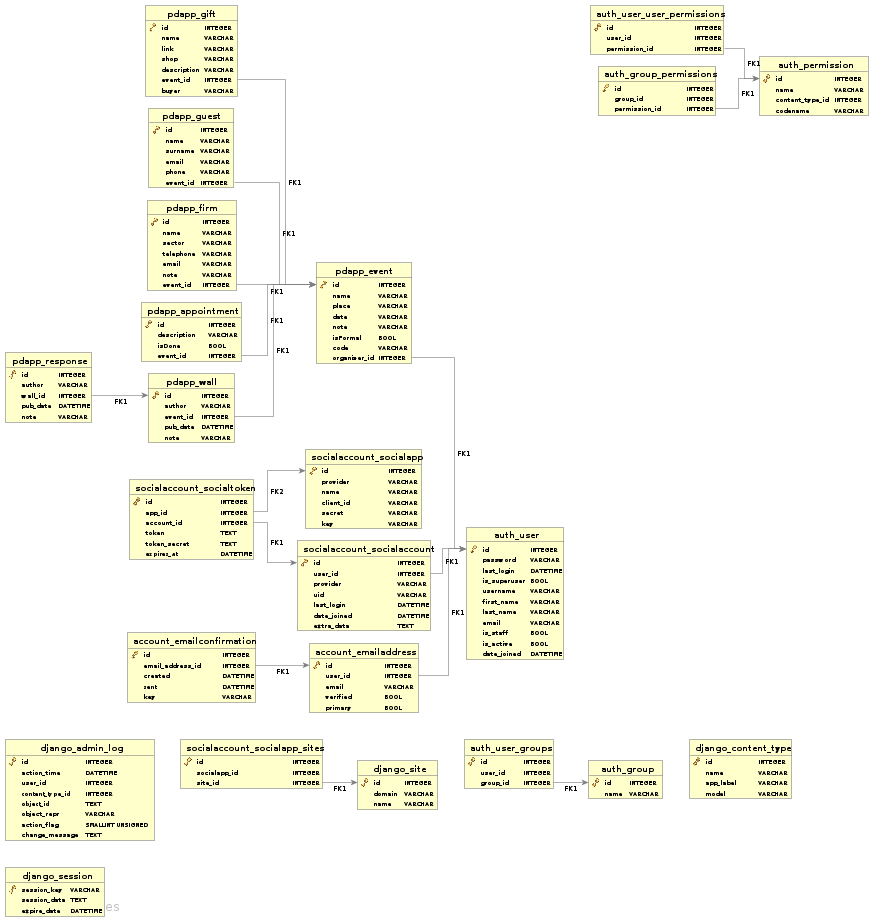
\includegraphics[scale=0.4]{/home/lagvna/Dokumenty/inz_gfx/dball.png}
 \caption{Diagram przedstawiający pełny schemat bazy danych, wraz z tabelami Django oraz wtyczki Allauth}
 \label{fig:db}
 \end{center}
\end{figure}

\end{appendices}




\end{document}
